\documentclass[twoside,11pt]{article}

\usepackage{graphicx}
\usepackage{booktabs}
\usepackage{tabularx}
\usepackage{array}
\usepackage{pdflscape}

% Any additional packages needed should be included after jmlr2e.
% Note that jmlr2e.sty includes epsfig, amssymb, natbib and graphicx,
% and defines many common macros, such as 'proof' and 'example'.
%
% It also sets the bibliographystyle to plainnat; for more information on
% natbib citation styles, see the natbib documentation, a copy of which
% is archived at http://www.jmlr.org/format/natbib.pdf

% Available options for package jmlr2e are:
%
%   - abbrvbib : use abbrvnat for the bibliography style
%   - nohyperref : do not load the hyperref package
%   - preprint : remove JMLR specific information from the template,
%         useful for example for posting to preprint servers.
%
% Example of using the package with custom options:
%
% \usepackage[abbrvbib, preprint]{jmlr2e}

\usepackage{jmlr2e}

% Definitions of handy macros can go here

\newcommand{\dataset}{{\cal D}}
\newcommand{\fracpartial}[2]{\frac{\partial #1}{\partial  #2}}

% Heading arguments are {volume}{year}{pages}{date submitted}{date published}{paper id}{author-full-names}

\usepackage{lastpage}
\jmlrheading{23}{2022}{1-\pageref{LastPage}}{1/21; Revised 5/22}{9/22}{21-0000}{Author One and Author Two}

% Short headings should be running head and authors last names

\ShortHeadings{Sample JMLR Paper}{One and Two}
\firstpageno{1}

\begin{document}

\title{Sample JMLR Paper}

\author{\name Author One \email one@stat.washington.edu \\
       \addr Department of Statistics\\
       University of Washington\\
       Seattle, WA 98195-4322, USA
       \AND
       \name Author Two \email two@cs.berkeley.edu \\
       \addr Division of Computer Science\\
       University of California\\
       Berkeley, CA 94720-1776, USA}

\editor{My editor}

\maketitle

\begin{abstract}
[TBD]
 
\end{abstract}

\begin{keywords}
  keyword one, keyword two, keyword three
\end{keywords}

\section{Introduction}
Digital health and clinical artificial intelligence increasingly depend on access to diverse, multimodal, and representative data distributed across organisations and care settings. Models developed or validated within a single institution may not perform consistently across different populations or operational contexts. Broader collaboration can therefore improve the robustness and generalisability of analytical systems while reducing dependence on narrowly defined local datasets [Li et al., 2025; Bradley et al., 2016; Trinh et al., 2025].  

Despite substantial investment in digital health and artificial intelligence, many initiatives that show promising results in pilot settings do not progress to sustainable operational services [Topol, 2019; Gandhi et al., 2024]. This transition is commonly discussed in terms of model performance, data quality, clinical validation, or local implementation barriers. A further difficulty arises when the collaboration itself must change. Adding a new organisation may require additional contracting, governance review, technical integration, and assurance. Similar concerns have been identified in large-scale health-data programmes, where organisational and technical integration can become major sources of delay [Goldacre \& Morley, 2022].  

A pilot can usually assume a predefined collaborative arrangement. The participating organisations, datasets, analytical objectives, and responsibilities are established before execution and remain relatively stable during the study. An operational service cannot make the same assumption. It must accommodate broader participation, more comprehensive data, and additional analytical capabilities as needs and circumstances change. The problem is therefore not only how to execute a distributed computation, but how to allow a governed collaboration to evolve without reconstructing its organisational and technical arrangements for every new activity. 

Existing health-data infrastructures address important parts of this problem. Centralised data platforms provide common custody and access mechanisms. Trusted Research Environments provide controlled analytical access to governed datasets. Federated learning frameworks allow computation to occur across organisational boundaries while keeping raw data local. Data-space and policy frameworks establish requirements for participation and data sovereignty. These mechanisms remain necessary, but they operate at different layers of a collaborative system. In particular, the decision that a new participant may enter a specific federated activity, under a defined authority, purpose, and set of capabilities, is often distributed across contracts, accreditation, identity systems, application configuration, and operational controls.  

OpenHealth addresses this transition from fixed collaboration to evolving service through Federated Computing. Rather than treating a collaboration as a collection of connected technical endpoints, Federated Computing represents it as a governed structure within which autonomous organisations retain sovereignty over their data and local systems while participating under shared constitutional rules. The objective is not to replace existing health-data platforms, identity systems, federated learning frameworks, or organisation-local security controls. It is to provide the governance structure through which new participation can become legitimate within an existing federation. 

A central mechanism in this structure is session-bound admission. Participation is not treated as a permanent property of an authenticated organisation or user. Instead, a participant is admitted to a specific governed activity for a defined purpose and with bounded capabilities. This allows different participation relations to coexist within the same federation. An organisation may contribute to a federated training activity without acquiring the same rights as an existing federation member, and permission to contribute does not automatically imply permission to consume the resulting model. 

This distinction is particularly relevant to the pilot-to-service transition. Collaboration growth need not mean adding increasingly many organisations with equivalent privileges. A federation can instead evolve by establishing new, purpose-specific participation relations while preserving its governance invariants. Such an approach may reduce the need to reconstruct governance arrangements whenever a new organisation, data source, or mode of participation is introduced. 

The OpenHealth demonstrator examines this proposition in a multisite federated learning setting using PathMNIST. An initial federation composed of Hospitals A and B is extended through the governed participation of Hospital C as a sponsored contributor. Hospital C is permitted to contribute to federated training while remaining unable to consume the resulting model. The implementation therefore provides a controlled setting in which to examine whether a federation can expand through asymmetric participation while maintaining explicit authority, capability boundaries, session binding, and auditable decision evidence. 

The study addresses the following research question: 

RQ: Can an open federated health infrastructure support the governed evolution of a collaboration by admitting new forms of participation while preserving bounded capabilities and auditable accountability? 

The paper makes three contributions. First, it reframes the transition from pilot to service as a problem of governed federation evolution rather than solely one of computational or data scale. Second, it presents an OpenHealth implementation of Federated Computing in which session-bound admission, capability separation, and auditable decision evidence are integrated with a conventional federated learning runtime. Third, it evaluates the approach through a controlled federation-expansion scenario in which an additional organisation contributes to model training without acquiring unrestricted federation rights. 

The remainder of the paper first reviews existing collaborative health-data approaches and the governance functions they provide. Section 3 introduces the Federated Computing principles used by OpenHealth. Section 4 describes the OpenHealth implementation and experimental demonstrator. Subsequent sections report the evaluation results, discuss implications for scalable health-data collaboration, and identify limitations and directions for further development. Section 5,    
  
% =============== Section 2 =================
\section{Existing Solutions and Related Work }

\subsection{Collaborative health-data infrastructures }

Health-data collaboration is supported by several classes of infrastructure that address different parts of the problem. These include centralised data platforms, Trusted Research Environments (TREs), proprietary federated platforms, open-source federated learning frameworks, and policy or data-sovereignty frameworks. They should not be considered direct substitutes. Each establishes a different boundary around data custody, computation, participation, and governance. 

Centralised data platforms simplify integration by bringing data under a common technical and administrative environment. Users and datasets can then be governed through repository-level identity, access-control, and data-management mechanisms. This model is effective where central custody is organisationally and legally acceptable, but it is less suitable when participating organisations must retain direct sovereignty over sensitive health data. The original OpenHealth analysis identified this dependence on central custody as the principal limitation for cross-organisational use cases in which data cannot simply be transferred into a common repository.  

Trusted Research Environments provide a different model. Rather than broadly centralising operational health-data services, they create controlled environments in which approved researchers or projects can analyse specified datasets under explicit governance and disclosure controls. OpenSAFELY is a prominent example of this approach. TREs provide strong mechanisms for research approval, controlled access, and accountability, but their principal governance object is generally access to existing datasets for approved research rather than the continuing evolution of a federation of autonomous organisations, resources, and operational relationships.  

Proprietary integration and federated platforms support cross-site analytics while allowing participating organisations to retain local data. Examples considered in the initial OpenHealth analysis include Rhino Health, Syntropy, and the Mayo Clinic Platform. Such platforms can provide substantial integration, governance, deployment, and operational functionality. Their participation model, however, is normally defined within the governance and technical environment of the platform itself. The relevant distinction for OpenHealth is therefore not whether these platforms provide governance — they do — but whether the rules by which participation changes are portable independently of the platform implementing the computation. 

Open-source federated learning frameworks, including Flower, NVIDIA FLARE, Intel OpenFL, PySyft, and Substra, provide the computational mechanisms required to execute distributed machine-learning workflows. They solve an important health-data problem by allowing model training across sites without requiring raw data to be collected centrally. Their principal abstraction, however, is the distributed computation. Decisions about which organisations may participate, under whose authority, and under which cross-organisational governance conditions are commonly established through deployment configuration and surrounding organisational processes. 

Finally, policy and data-sovereignty frameworks, including Gaia-X, the European Health Data Space (EHDS), and TEHDAS, address requirements for trustworthy data sharing, organisational eligibility, interoperability, and data sovereignty. These frameworks provide important institutional and regulatory conditions under which data collaboration can occur. They operate at a different level from the runtime mechanisms that determine whether a particular participant may undertake a particular federated activity. 

These approaches therefore address complementary parts of the same health-data collaboration problem. The OpenHealth question is not which one should be replaced, but how their respective functions can coexist when a collaboration must evolve. 

\subsection{Identity and operational access control }

Cross-organisational infrastructures also depend on established identity and access-control mechanisms. Federated identity systems can authenticate principals across organisational boundaries, while OAuth-based mechanisms, cloud IAM, RBAC, and ABAC can control access to services and resources. 

These technologies are necessary deployment foundations. They answer questions such as whether an identity can be trusted, whether a service account may invoke an API, or whether a user possessing particular attributes may access a resource. 

The difficulty arises when such mechanisms also become the implicit representation of the collaboration itself. 

In practical deployments, session participation can become distributed across cloud IAM policies, platform configuration, central policy services, and checks embedded in orchestration code. This makes cross-organisational integration increasingly bespoke because participating organisations have heterogeneous identity and deployment stacks. It also makes past decisions difficult to reconstruct and allows operational configuration changes to modify effective admission behaviour over time.  

The distinction is therefore between organisation-local access control and the cross-organisational decision that establishes participation in a shared activity. 

Session admission determines whether a participant may enter the collaborative session, whereas organisation-local IAM continues to determine what actors may do within their respective organisational environments after entry.  

OpenHealth adopts the same separation but applies it to a broader health-data federation rather than only to the interface of a federated learning session. 

\subsection{Federated learning and session admission }

Federated learning is particularly relevant to OpenHealth because it demonstrates both the value and the limitations of computational federation. 

In cross-silo FL, multiple organisations train a shared model while retaining raw data locally. The FL framework coordinates operations such as model distribution, local training, update submission, aggregation, and evaluation. The computational procedure can therefore be federated even when organisational governance remains external to it. Each request is associated with a specific collaborative session, permitted operation, and holder identity, and produces an explicit ALLOW or DENY decision together with structured evidence. The underlying Flower training and aggregation procedure remains unchanged.  

This is an important precedent for OpenHealth for two reasons: (i) first, it demonstrates that governance of participation can be separated from the analytical framework executing the work; (ii) second, it demonstrates that such governance need not remain an administrative declaration. It can become an executable boundary whose behaviour is tested through both successful and denied requests. 

OpenHealth extends this idea beyond the original FLICS setting. The concern is no longer only which operation a predefined participant may invoke within an FL session. The broader question is how the federation itself can accommodate new forms of participation while preserving its governing conditions. 

\subsection{Data interoperability and semantic models }

Cross-organisational health-data collaboration also requires semantic interoperability. Different institutions may use different data structures, terminologies, coding systems, and representations of clinically equivalent concepts. Shared vocabularies, information models, and ontologies can therefore play an important role in making distributed data interpretable across organisational boundaries. 

This problem is complementary to federation governance. A semantic ontology can specify that concepts represented differently by two hospitals refer to the same clinical entity or relationship. It does not determine whether one hospital is entitled to contribute those data to a particular collaborative activity, whether another participant may use the resulting model, or under whose authority either operation occurs. 

OpenHealth therefore distinguishes semantic interoperability of resources from governance of participation. Both may be necessary in a production health-data service, but they solve different problems. The federated governance layer does not require participating organisations to surrender their internal data models, nor does an agreed semantic model itself establish federation rights. 

\subsection{ Data spaces and organisational sovereignty }

Policy-oriented data-space initiatives provide another important part of the surrounding landscape. Their emphasis on sovereignty, trustworthy exchange, conformity, and organisational eligibility is closely aligned with the requirement that health organisations retain control over their resources while collaborating. 

Data-space frameworks can establish the conditions under which an organisation or service is eligible to participate in a wider ecosystem. OpenHealth addresses the narrower operational transition from such eligibility or organisational agreement to participation in a particular governed activity. 

Eligibility therefore does not automatically imply admission to every activity. Conversely, a federation-level admission decision does not replace the regulatory, contractual, ethical, or organisational requirements that established eligibility in the first place. 

This layered interpretation avoids treating technical admission as a substitute for institutional governance. OpenHealth instead provides a means by which agreed governance conditions can become executable at the federation boundary. 

\subsection{AI-agent frameworks and runtime orchestration }

Emerging agent frameworks add a further form of computational participation. Their principal concern is how an AI-driven process performs tasks through tools, services, workflows, memory, or other computational resources. Such frameworks can provide their own runtime controls, including tool restrictions, isolation, approval mechanisms, and monitoring. 

From the perspective of OpenHealth, these are operational mechanisms. The federation-level question remains whether the computational participant is entitled to invoke a particular federated capability, under which organisational authority, for which purpose, and within which governed context. 

This distinction prevents the federation architecture from becoming dependent on a particular agent implementation. An agent framework can change without changing the governance semantics of the federation, just as the Flower runtime can be replaced without changing the principle of session-bound admission. 

Section 4 applies this distinction explicitly to AI-agent participation and considers how admission and runtime conformance complement agent-specific containment and execution mechanisms. 

\subsection{Comparative view }

Table 1 summarises the different functions provided by the principal approaches discussed above. The comparison is deliberately functional rather than competitive. A checkmark does not imply that a function is implemented identically across products or deployments, and the table is not intended as a feature ranking 


\begin{landscape}

\begin{table}[htbp]
\centering
\scriptsize	
\caption{Functional comparison of approaches supporting cross-organizational health-data collaboration.}
\label{tab:existing-solutions}
 
\begin{tabularx}{\linewidth}{
    >{\raggedright\arraybackslash}p{2.8cm}
    >{\raggedright\arraybackslash}p{2.4cm}
    >{\raggedright\arraybackslash}p{2.4cm}
    >{\raggedright\arraybackslash}p{2.0cm}
    >{\raggedright\arraybackslash}p{2.4cm}
    >{\raggedright\arraybackslash}p{2.4cm}
    >{\raggedright\arraybackslash}p{2.4cm}
}
\toprule
\textbf{Approach} &
\textbf{Primary governance boundary} &
\textbf{Data remain under organizational control} &
\textbf{Controls operational access} &
\textbf{Establishes purpose-specific participation} &
\textbf{Participation decision externally auditable} &
\textbf{Supports governed change of participation} \\
\midrule

Centralized data platforms: enterprise cloud data lakes (Runyon, 2022)
&
Repository / data controller
&
Usually no
&
Yes
&
Deployment dependent
&
Deployment dependent
&
Through repository governance
\\

\addlinespace

Trusted Research Environments (TREs): OpenSAFELY
(opensafely.org; Williamson et al., 2020; Kavianpour et al., 2022)
&
Approved project / research environment
&
Often logically controlled by custodian
&
Yes
&
Yes, for approved research
&
Yes
&
Primarily through new project / governance approval
\\

\addlinespace

Proprietary federated platforms: Rhino FCP, Syntropy, Mayo Clinic Platform
&
Platform federation
&
Yes
&
Yes
&
Platform dependent
&
Platform dependent
&
Platform dependent
\\

\addlinespace

Open-source federated learning frameworks: Flower, NVIDIA FLARE,
Intel OpenFL, PySyft, and Substra
&
Federated computation
&
Yes
&
Runtime dependent
&
Usually external to FL framework
&
Usually external
&
Usually external
\\

\addlinespace

Data-space / sovereignty frameworks: Gaia-X, EHDS, and TEHDAS
&
Ecosystem eligibility and exchange
&
Yes
&
Implementation dependent
&
At policy / ecosystem level
&
Governance dependent
&
Yes, principally at ecosystem level
\\

\addlinespace

\textbf{OpenHealth / Federated Computing}
&
{Governed federation activity}
&
\textbf{Yes}
&
Complementary local / runtime mechanisms
&
{Explicit and session-bound}
&
{Explicit decision evidence}
&
{Through bounded participation relations}
\\

\bottomrule
\end{tabularx}

\end{table}

\end{landscape}

The principal difference shown by Table 1 is therefore not that existing approaches lack governance. Rather, governance is located at different boundaries. 

Centralised platforms govern the repository. TREs govern approved research access. Federated learning frameworks govern distributed computation but commonly rely on surrounding systems for organisational participation. Data-space frameworks govern ecosystem-level conditions. Organisation-local IAM governs identities, services, and resources within a participant's administrative domain. 

OpenHealth introduces an additional boundary at the point where a proposed participant enters a particular governed federated activity. 

This boundary is intended to compose with the mechanisms above rather than displace them. 

\subsection{Gap addressed by OpenHealth }

The related work suggests a narrower gap than the original claim that existing infrastructures simply “do not provide admission”. 

The unresolved problem is the transition between institutional agreement and operational participation when the collaboration changes. 

A health organisation may already be authenticated. It may satisfy regulatory or data-space eligibility requirements. Its infrastructure may be technically interoperable with a federated learning platform. Its users may possess valid local permissions. None of these conditions alone determines whether that organisation, user, or computational process should participate in a particular federated activity with a specified purpose and bounded capability. 

OpenHealth addresses this transition by making the participation decision explicit, session-bound, and auditable while leaving data custody, local identity, operational authorization, and analytical execution with the mechanisms best suited to those functions. 

The next section describes how Federated Computing provides the governance model required to make this separation operational. 

\subsection{Dimensions of Collaboration Growth }

Scaling a collaboration requires the ability to change not only the number of participating organisations, but also the resources available to the federation and the operations that participants may perform. These changes are governed differently and should not be conflated. New organisations establish new participation relations, new datasets or models extend the federation’s resource base, and new analytical capabilities extend the set of permitted operations. OpenHealth therefore treats scaling as governed evolution across participants, resources, and operations rather than as the admission of a single class of heterogeneous entities. 

\begin{table}[htbp]
\centering
\caption{Dimensions of collaboration growth and their associated governance questions.}
\label{tab:collaboration-growth}

\begin{tabularx}{\textwidth}{
    >{\raggedright\arraybackslash}p{3.0cm}
    >{\raggedright\arraybackslash}p{5.0cm}
    >{\raggedright\arraybackslash}X
}
\toprule
\textbf{Dimension of evolution} &
\textbf{What changes} &
\textbf{Governance question} \\
\midrule

Participation
&
Organisations, human or computational participants, including AI agents
&
Under whose authority may they participate?
\\

\addlinespace

Resources
&
Datasets, models, compute, analytical services
&
Under what conditions may they be contributed, exposed, or used?
\\

\addlinespace

Operations
&
Training, inference, validation, analysis
&
Which activities are permitted, for which purpose and scope?
\\

\bottomrule
\end{tabularx}

\end{table}


These dimensions are related but not interchangeable. Scaling therefore requires governed changes in relations among participants, resources, and operations rather than the admission of a single heterogeneous class of entities. 
% ==================== section 3 ===================

\section{OpenHealth as a Federated Computing Infrastructure }

\subsection{The governance problem behind collaboration growth }

Moving a health data collaboration from a pilot towards an operational service requires more than scaling its computation. A pilot can usually begin with a predefined group of organisations, datasets, responsibilities, and analytical objectives. These arrangements can be negotiated and configured before the pilot starts. A service, however, must accommodate change. New organisations may contribute data, existing participants may assume new roles, additional analytical resources may become available, and different forms of participation may be required for different purposes. 

Federated learning addresses an important part of this problem by allowing organisations to collaborate without transferring their raw data to a common repository. It does not, by itself, determine under whose authority a new participant may enter a collaboration, which activities that participant may perform, for which purpose, or how such a decision can later be justified. 

In operational cross-organisational systems these questions are commonly distributed across identity systems, access-control rules, contractual arrangements, application configuration, and orchestration logic. The resulting arrangement can work for a fixed collaboration, but becomes increasingly difficult to maintain when the collaboration changes. Different organisations operate different identity, policy, and infrastructure stacks; changes can require bespoke integration; and the reason why a particular activity was permitted may later need to be reconstructed from several independent systems. Similar problems have been identified for cross-silo federated learning, where configuration and organisation-specific IAM provide necessary controls but do not by themselves provide portable, session-scoped admission semantics and boundary-visible evidence.  

OpenHealth therefore treats collaboration growth as a federation governance problem, rather than solely as a data-integration or machine-learning problem. 

\subsection{Federated Computing }

OpenHealth is based on Federated Computing, a model in which autonomous organisations collaborate without surrendering sovereignty over their local resources and operational systems. The federation provides a common governance structure for the collaboration while individual organisations retain control of their own data, infrastructure, identities, and internal access mechanisms. 

This produces an important architectural separation. Local mechanisms answer organisation-specific questions such as which hospital employee may access a local system, which service account may invoke an internal API, or how local data are protected. The federation answers the cross-organisational question of whether a proposed form of participation is legitimate within the governed collaborative context. 

Federated Computing therefore complements rather than replaces existing mechanisms. Identity federation, IAM, RBAC or ABAC, Trusted Research Environments, federated learning frameworks, and local security controls remain applicable inside their respective domains. The additional function is a common boundary at which participation in a federated activity can be evaluated before the activity is executed. 

This separation was demonstrated in the FLICS architecture for cross-silo federated learning. There, session admission governs the transition into a collaborative FL session while conventional organisation-local IAM continues to govern activity within each participating organisation. OpenHealth generalises this principle to a health-data federation in which different organisations may participate under different governed relationships. 

\subsection{Federation as a governed context }

A central feature of the OpenHealth approach is that participation is not treated as a permanent property of an organisation simply because that organisation has been authenticated or previously approved. 

Instead, participation is established within a specific governed context. Before computation begins, the federation establishes the applicable governance conditions. These conditions determine the participating authorities, purpose of the collaboration, applicable policy, and permitted forms of participation. OpenHealth represents this bounded context through a federation envelope. 

Capabilities issued within that context describe what a participant may request. The admission boundary then determines whether the proposed participation is consistent with the governed context before the corresponding activity is allowed to proceed. 

The resulting architecture separates three concerns that are frequently collapsed in operational systems: governance establishment → capability expression → operational execution. The first establishes the conditions under which the collaboration exists. The second expresses the bounded activities available to a participant. The third performs the actual computation. This is particularly useful when a collaboration must evolve. Changing the set of participants does not require redefining the entire operational environment. Instead, the federation determines whether the new participation relation is compatible with its existing governance conditions. 

\subsection{Session-bound admission }

OpenHealth implements this principle through session-bound admission. Admission occurs at the transition between federation setup and the activity being requested. It answers a narrower question than general access control: May this participant perform this federated activity, for this purpose, within this governed session? The decision is explicit and produces either an ALLOW or DENY outcome before the requested computation proceeds. 

This boundary-oriented design follows the same basic principle validated in FLICS, where session-interface requests are evaluated against session-specific capabilities and explicit decision records are generated for both successful and unsuccessful requests. FLICS showed that such checks can be placed at the collaborative boundary without changing the underlying federated learning procedure.  

OpenHealth retains this separation but embeds it within a broader federation-governance workflow. The governed session is established first; capabilities are subsequently issued within that context; and the gatekeeper evaluates requests before allowing the corresponding operational workflow to proceed. 

The federated learning framework remains responsible for training and aggregation. It does not determine the governance legitimacy of the participant entering that activity. 

\subsubsection{ Admission of participants }

 [TBD]

\subsubsection{Admission of AI Agents }

The same federation-governance problem applies when participation is performed by an AI agent rather than directly by a human user or conventional software client. 

Contemporary agent frameworks such as OpenClaw provide environments in which an AI agent can invoke tools, load reusable skills, interact through multiple channels, and extend its runtime capabilities through plugins. Other agent frameworks provide related abstractions for tool use, multi-agent orchestration, handoffs, guardrails, and persistent execution state. These mechanisms determine how an agent acts once it is running. 

OpenHealth addresses a different question: Under what authority may an AI agent participate in a governed health-data federation, for which purpose, and with access to which federated capabilities? An agent is therefore not treated as a new governance category parallel to organisations, datasets, or models. From the perspective of the federation, it is a computational participant acting under an accountable organisational relationship. Its internal architecture, model provider, planning strategy, memory system, or agent framework does not determine its federation rights. 

Before an agent can invoke a federated operation, OpenHealth applies the same session-bound admission principle used for other participants. The agent must present a valid capability bound to the current governed federation context. The gatekeeper evaluates the requested operation, purpose, scope, and holder binding before the request is allowed to reach the corresponding operational service. 

This creates an explicit separation between agent runtime capability and federation capability. For example, an OpenClaw deployment may locally possess tools capable of file access, network communication, API invocation, or other actions. Such local capabilities do not imply that the agent is entitled to invoke resources inside an OpenHealth federation. Conversely, admission to a bounded federation operation does not grant the agent unrestricted access to its local or external runtime environment. 

The distinction is analogous to that already made between Federated Computing and federated learning. Flower determines how federated training is executed after participation has been admitted. An agent framework determines how an AI agent reasons, invokes tools, and coordinates actions after execution begins. In both cases, OpenHealth governs the cross-boundary participation relation. 

This separation also avoids making assumptions about agent autonomy or predictability. Admission does not certify that an AI agent will behave correctly during execution. Runtime mechanisms such as tool policies, sandboxing, network isolation, human approval, guardrails, monitoring, or agent-specific security controls remain complementary. Contemporary agent frameworks already provide some of these controls. For example, the OpenAI Agents SDK supports tool and workflow guardrails, approvals, sandboxed execution, and handoffs. OpenClaw similarly provides policies governing tool exposure and runtime capabilities.  

The role of OpenHealth is prior and narrower. It determines whether the computational participant may cross the federation boundary for the requested activity. In the proof-of-concept architecture, this allows an AI agent to be treated as another mode of participation without modifying the federation model. A human user, a conventional client process, or an AI-driven process can all request a federated capability. What differs is the capability granted and the operational controls applied after admission, not the constitutive governance mechanism itself. This property is important for future health-data services because agent technologies are likely to change rapidly. Binding federation governance to a particular agent framework would therefore make the infrastructure dependent on transient implementation choices. By placing admission outside the agent runtime, OpenHealth can admit an agent implemented using OpenClaw, the OpenAI Agents SDK, AutoGen, or another framework without changing the federation's governance model. 

Recent agent incidents illustrate a less visible problem. Assurance properties are difficult to observe when systems behave as expected and become apparent only when an operational boundary is crossed. Such events are commonly interpreted primarily as failures of model reliability or agent behavior. This interpretation can obscure a prior systems question: whether the effective capabilities available to the computational participant were consistent with the authority, purpose, and scope under which it was allowed to participate. OpenHealth makes this distinction explicit. Admission defines the permitted participation relation, while a conformance criterion requires the operational environment exposed to the participant to remain consistent with that relation. A violation can therefore be identified not simply as unexpected agent behavior, but as a failure of the system to preserve an asserted governance boundary. This is particularly important for AI agents because their runtime behavior may vary while the federation's assurance obligations must remain stable. 

 

\subsection{ Differentiated participation }

This architecture also avoids the assumption that collaboration growth requires adding increasingly many equivalent members. 

Different organisations can establish different relations with the federation. 

An existing federation member may have capabilities associated with training and model use. Another organisation may be permitted only to contribute to a specific federated training activity. A computational participant may eventually be admitted for another narrowly defined operation. These forms of participation need not confer equivalent rights. 

This is particularly relevant to health-data collaboration, where willingness to contribute a resource does not necessarily imply a reciprocal right to consume every resource generated by the collaboration. 

OpenHealth therefore separates participation from capability. Being permitted to contribute does not automatically imply permission to query a model. Being admitted to one activity does not establish unrestricted participation in other activities. Sponsorship similarly provides an accountable route through which a new participant may be considered by the federation without transferring the sponsor's own rights to that participant. 

The practical consequence is that a federation can grow through asymmetric but explicitly governed relationships rather than requiring every new organisation to become an identical member. 

This property is central to the proof of concept described in Section 4, in which Hospital C is permitted to contribute to federated training without acquiring the model-consumption capabilities available to the existing federation members. 

\subsection{Governance as auditable evidence }

A further requirement for collaboration at service scale is the ability to explain how participation decisions were made. 

When authorization is distributed across application configuration, cloud IAM rules, orchestration services, and local systems, reconstructing a past decision can require recovering the configuration state of several components. FLICS addressed this problem by producing an explicit structured record for every admission decision, including the session, operation, outcome and reason for the decision. Its evaluation showed that denied requests as well as admitted requests could be reconstructed from boundary-visible evidence after execution.  

OpenHealth adopts the same evidence-oriented principle. An admission decision is therefore not merely a transient control action. It becomes a governance artefact associated with the context in which participation was requested. The evidence records who requested the activity, the relevant capability and purpose, whether the request was admitted, and the reason for that decision. 

This provides a direct link between governance intent and operational participation without requiring the federation to centralise the participating organisations' internal policy systems. 

\subsection{Why this matters for OpenHealth }

Federated Computing addresses three practical requirements that become increasingly important as OpenHealth moves from a fixed proof of concept towards a reusable health-data infrastructure. 
\begin{itemize}
    \item First, it provides a common governance boundary across heterogeneous organisations while allowing each organisation to retain its own identity, infrastructure, and data-management mechanisms. 

\item  Second, it allows the federation to change its participation structure without granting uniform rights to every new participant. Capabilities can reflect the specific purpose for which an organisation participates. 

\item  Third, it makes the decision to participate explicit and auditable before computation, rather than leaving that decision implicit in application configuration or reconstructing it retrospectively from runtime logs. 
\end{itemize}

The result is not another federated learning framework. Federated Computing provides the governance structure within which technologies such as Flower can be used. OpenHealth applies that structure to the practical problem of extending a health-data collaboration while preserving organisational sovereignty, bounded participation, and accountability. 

Section 4 describes the implementation of these principles in the OpenHealth proof of concept. 

% ===================== Section 4 ======================
\section{OpenHealth PoC Implementation }

\subsection{System architecture }

The OpenHealth proof of concept (PoC) implements a governed federated learning environment in which participation is established for a specific federation session before computation begins. The implementation separates the governance and admission plane from the federated learning runtime. This allows the conditions under which an organisation or actor participates to be evaluated independently from the technology executing the subsequent computation. 

The architecture contains four functional areas: 
\begin{enumerate}
    \item the user and federation-authority interfaces  
\item the OpenHealth governance and orchestration services  
\item the federated learning runtime  
\item the participating hospital sites  
\end{enumerate}

The separation between these areas is intentional. OpenHealth does not replace the federated learning framework. Flower remains responsible for distributed model training and aggregation. OpenHealth determines whether participation in a particular federation session is legitimate and under which capabilities that participation may occur. 

Figure 1 presents the proof-of-concept architecture using a C4-style container view. 

\begin{figure}[htbp]
    \centering
    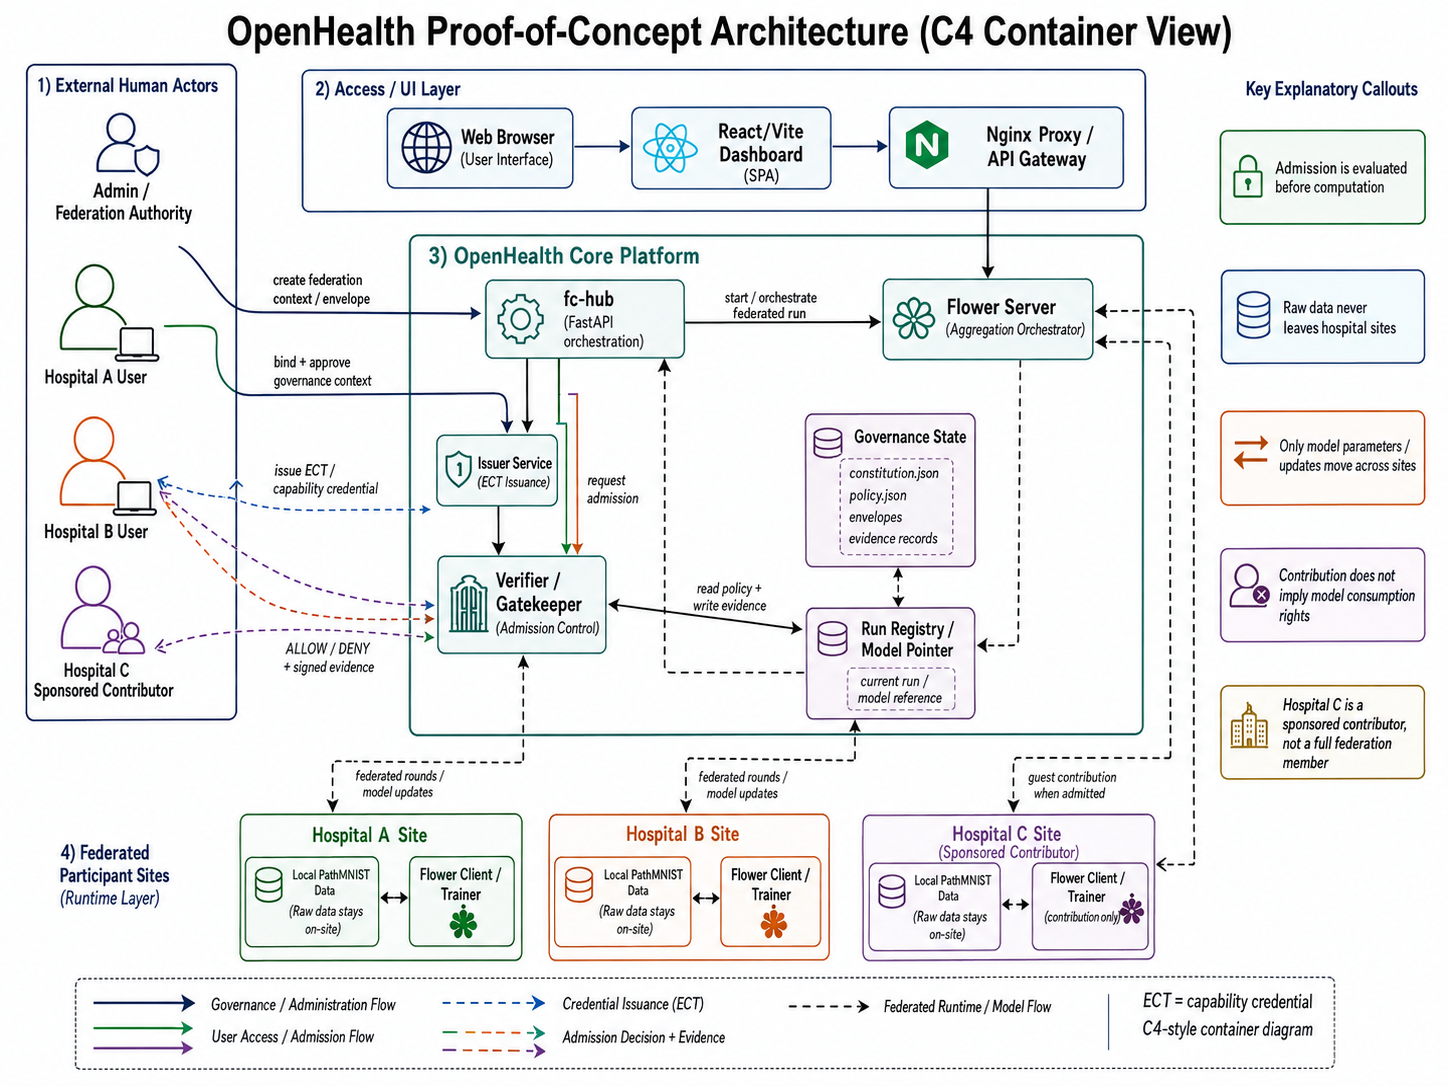
\includegraphics[width=\textwidth]{Fig1_Architecture.png}
    \caption{
        OpenHealth proof-of-concept architecture.
        The governance and admission layer establishes session-bound
        participation before execution by the federated learning runtime.
        Hospitals retain their PathMNIST data locally, while the Flower
        runtime exchanges model updates rather than raw data.
        Hospital C participates as a sponsored contributor with a capability
        restricted to federated training; successful contribution does not
        confer model-consumption rights.
    }
    \label{fig:openhealth-architecture}
\end{figure}


\subsection{Federation context and session-bound admission }

Admission in OpenHealth is not a persistent statement that an actor is generally trusted or authorised. It is evaluated relative to a specific governed federation context. 

Before a federated activity begins, the federation authority creates an envelope representing the session-specific governance context. The envelope identifies the context in which subsequent participation decisions are valid and binds the activity to the applicable constitutional and policy state. 

The envelope\_id therefore acts as the admission binding for the session. This distinction is central to the implementation. Authentication establishes who an actor is. A capability credential represents what that actor may request. Neither independently establishes the right to participate in an arbitrary federated activity. Admission is evaluated when the capability is presented within the governed context identified by the envelope. 

The resulting relation can be expressed conceptually as: identity + capability + governed session context → ALLOW or DENY. The decision is consequently contextual rather than global. A capability valid for one federation context does not imply unrestricted participation outside that context. 

This is what makes the mechanism session-bound admission rather than conventional account-level access control. 

\subsection{Governance establishment }

The federation authority establishes the governance context before operational execution. In the proof of concept, this process includes creation of the envelope and explicit binding and approval of the governance context. The approval process is protected by the governance mechanisms implemented in OpenHealth, including the KYO-based binding procedure and the required approvals. 

The resulting governance state provides the basis against which later admission requests are evaluated. The governance state contains the relevant constitutional and policy information together with the active envelopes and the evidence generated by admission decisions. These artefacts are maintained independently from the Flower runtime. This separation preserves an important architectural invariant. The runtime does not define the legitimacy of participation. It executes computation only after that legitimacy has been established by the governance layer. 

\subsection{ Capability issuance }

Participants interact with the federation through explicitly issued capability credentials. The OpenHealth issuer service produces an ECT, the capability credential used by the proof of concept. The ECT is bound to the relevant governance context and expresses the capabilities available to the holder, including the permitted resource, operation, purpose, and applicable scope. 

The ECT is not itself an admission decision. It provides evidence that a participant possesses a capability that may be presented for admission. The gatekeeper subsequently evaluates that capability in the context of the requested activity. This distinction prevents capability issuance from becoming equivalent to unrestricted federation membership. A participant may therefore hold a narrowly scoped capability without acquiring other capabilities available to existing federation members. We exploit this property directly in the Hospital C experiment. 

\subsection{ Admission gateway }

The verifier and gatekeeper constitute the admission boundary of the OpenHealth proof of concept. When a participant requests entry into a governed activity, the gatekeeper evaluates the request against: 
\begin{itemize}
    \item the participant identity  

 \item the presented ECT  

 \item the envelope\_id  

 \item the requested operation  

 \item the stated purpose  

 \item the requested resource and scope  

 \item the applicable policy and constitutional state  
\end{itemize}

The result is an explicit ALLOW or DENY decision produced before the requested computation is executed. 

The gatekeeper also generates evidence describing the decision and its reason. Consequently, both successful and unsuccessful admission attempts become observable governance events rather than implicit outcomes of runtime configuration. 

This is different from authenticating a Flower client or checking a role after execution has already entered the federated runtime. The OpenHealth decision establishes whether that participant may enter the specified activity at all. 

\subsection{User and orchestration layer }

Users interact with the proof of concept through the React/Vite dashboard that separates federation administration from participant operations. Requests are routed through the Nginx gateway to the corresponding OpenHealth services. 

The fc-hub FastAPI service provides the orchestration layer. It coordinates the governed workflow and maintains the association between the current federation context and the operational federated-learning run. 

The orchestration layer does not itself determine policy. Admission decisions remain the responsibility of the verifier and gatekeeper. 

Similarly, the dashboard is not the source of governance truth. It exposes the state and operations of the underlying services. 

This distinction is important because the PoC is intended to demonstrate governance enforced by the system rather than governance represented only in a user interface. 

\subsection{Governance state and evidence }

Governance state is maintained separately from the federated model and training runtime. 

As illustrated in Figure 1, the verifier has access to the constitutional and policy artefacts required for admission evaluation. The implementation also maintains the active federation envelopes and the resulting decision evidence. 

For every evaluated request, the evidence record captures the relevant decision context, including the actor, requested capability, purpose, scope, decision outcome, and reason. 

The evidence trail therefore allows a later observer to distinguish: 
\begin{itemize}
    \item who requested participation  

\item under which governed session  

\item for which operation  

\item for which purpose  

\item with which capability  

\item whether participation was admitted  

\item why the decision was reached  
\end{itemize}

This evidence is produced by the admission process rather than inferred retrospectively from application logs. 

That is an important part of the PoC claim. 

 

\subsection{Run registry and model association }

The proof of concept maintains an explicit association between the governed federation context and the corresponding model run. 

The run registry and model pointer shown in Figure 1 identify the operational model associated with the current federated activity. This allows the governance layer and the federated runtime to remain separate while retaining a traceable relationship between them. 

The distinction between session admission and model execution is deliberate. 

The capability credential is bound to the governed federation context rather than being treated as an unrestricted token for arbitrary future model runs. Where a request concerns a particular executed run, the corresponding admission decision can additionally record that run association. 

This avoids collapsing three different concepts into one object: 

governed session, capability, and executed model run. 

 

\subsection{Federated learning runtime }

Once the required participation has been admitted, the operational computation is performed using Flower. 

The Flower server coordinates federated training rounds and aggregates updates received from participating clients. Each hospital operates its own Flower client and trainer. 

PathMNIST data remain within the corresponding hospital environment. The federated workflow exchanges the information required for model training rather than transferring the underlying raw images between participating hospitals. 

The Flower runtime is therefore intentionally conventional. 

The contribution of OpenHealth is not a new federated learning algorithm. It is the governance structure surrounding participation in that computation. 

This architectural separation also makes the approach potentially applicable to analytical runtimes other than Flower. 

 

\subsection{ Baseline federation }

The initial experimental configuration consists of Hospitals A and B. 

Both participate as federation members and operate local PathMNIST partitions. Their Flower clients contribute to the federated training workflow according to the capabilities established by the federation. 

This configuration provides the A+B baseline. The corresponding model is trained without data from Hospital C and provides the reference against which the later federation expansion is evaluated. 

The data partitioning intentionally results in weaker representation of selected PathMNIST classes (colon cancer data vs normal tissue) in the A+B configuration. This gives the later Hospital C contribution an observable analytical role rather than making the additional participant merely decorative. 

 

\subsection{Sponsored contribution by Hospital C }

The second configuration introduces Hospital C without converting it into an equivalent federation member. 

Hospital C participates through a sponsorship relation established by an existing federation participant. The sponsored contributor receives a capability permitting participation in federated training through the submit\_update operation for the specified training purpose. 

The capability does not include model-consumption rights. Consequently, the following two propositions are simultaneously true: 

Hospital C may contribute to the federated model. 

Hospital C may not query or consume that model merely because its contribution was admitted. 

This asymmetric participation relation is intentional. 

It demonstrates that federation growth need not be implemented by adding progressively more actors with identical privileges. OpenHealth permits a collaboration to expand through differentiated relations whose capabilities correspond to their purpose. 

The Hospital C experiment therefore tests more than technical onboarding. It tests whether the federation can change its participation structure while preserving explicit capability boundaries. 

 

\subsection{Controlled A+B versus A+B+C experiment }

The proof of concept compares three federation configurations. 

\subsubsection{A+B baseline }

Hospitals A and B train the federated model using their local PathMNIST partitions. 

\subsubsection{A+B+C governed expansion with a sponsred guest (Mode 1A) }

Hospital C participates as a sponsored contributor after successful session-bound admission and contributes additional training data while retaining its restricted capability set. 

Hospital C was allocated substantial representation of selected PathMNIST classes that were intentionally weakly represented in the A+B baseline. The expanded federation therefore provides a controlled means of examining whether a governed change in participation produces an observable change in the resulting model. 

The experiment has two independent outcomes: (i) The first is a governance outcome. Hospital C must be capable of contributing while remaining unable to perform operations outside its granted capability; (ii) the second is an analytical outcome. The A+B+C model can be compared with the A+B baseline to determine whether the additional data contribution alters model performance. These outcomes must not be conflated. Improved model performance does not validate the governance mechanism, and successful governance does not imply improved clinical performance. 

\subsubsection{ A+B+C governed expansion with an AI agent guest (Mode 1B)} 

[TBD] 

Mode 1B scenario is intended to make this otherwise invisible property observable. The agent is admitted for a narrowly bounded inference capability, while its runtime environment is constructed so that alternative paths to federation governance services or privileged operations are unavailable. The experiment therefore tests not whether the agent is intrinsically “safe” or that can be bound, but whether the system remains conformant with the participation relation that the federation admitted. If the agent attempts to escape outside that relation, the relevant question becomes whether the architecture prevents the attempt from acquiring effects beyond the admitted boundary. 

\subsection{What the proof of concept establishes }

The PoC is designed to establish three architectural properties: (i) First, federation participation can be made session-specific rather than treated as a persistent property of an authenticated actor; (ii) second, a federation can expand through asymmetric participation relations. A contributor need not acquire the rights of a full member; (iii) third, admission decisions can be made before computation and retained as explicit evidence linked to the governed context in which they were made. 

The experiment does not evaluate clinical effectiveness, production-scale deployment, or general health-system outcomes. Those questions remain outside the scope of this PoC. 
% ======================== ACK ============================
\acks{All acknowledgements .}

% Manual newpage inserted to improve layout of sample file - not
% needed in general before appendices/bibliography.

\newpage

 


\vskip 0.2in
\bibliography{sample}

\end{document}
